\documentclass[a4paper,11pt]{article}

\usepackage[nodayofweek]{datetime}
\longdate
\usepackage{algorithm}
\usepackage{algpseudocode}
\usepackage{graphicx}
\usepackage{enumitem}
\usepackage{fancyhdr}
\usepackage{float}
\usepackage{array}
\usepackage{multirow}
\usepackage{amsmath}
\usepackage{textcomp}
\usepackage{tabularx,ragged2e,booktabs,longtable,multirow,subfigure,caption}
\usepackage{hyperref}
\usepackage{url}
\usepackage{fancyhdr}
\usepackage[a4paper,hmargin=2.8cm,vmargin=2.0cm,includeheadfoot]{geometry}

\begin{document}

Abstract

\section {Introduction}

\subsection{Motivation}
On a general purpose CPU, the instructions of a program are carried out using a control flow model where the instructions are loaded into memory and each instruction is decoded and then executed by the processor. There also exists specialized technologies such as field-programmable gate arrays (FPGAs) and graphics processing units (GPUs). Each specialised technology has a different architecture that allows for some processes to be executed at an accelerated speed when compared to a CPU. Heterogeneous computing architectures refers to systems that use multiple types of processors\cite{heterogeneous}.
\\\\ 
A flexible application may be run in many different ways over a heterogenous system. Each of these options has its own cost, performance and usage characteristics\cite{harness}. The cost is defined as the amount of resources used. The performance of an application is measured by the volume of tasks processed per unit time. The usage characteristic of a platform is how the application will be deployed on the platform (i.e. different processors may have a different way of executing a process because of its architecture). It is important to know which platform configuration is best suited to an application's needs and hence, the performance of each platform configuration for the application has to be known. However, in order to evaluate the performance for a certain platform on an application, some form of experimentation is required. 

\subsection{Objectives}
The main aim of this project is to find a general method for deriving a simulation model that can predict the performance of an application on reconfigurable platforms. This allows the user to freely change the parameters of the model such as computing power and types of processors used to see how the performance is affected by these factors. Thus, allowing the application to run on a platform configuration that best suits its needs.


\section{Background}

\subsection{Related work}
The Hardware and Network-Enhanced Software Systems for Cloud Computing (HARNESS)\cite{harness} project proposes an enhanced cloud software stack that not only incorporates a wide variety of specialised technologies but also embraces the heterogeneity that those technologies bring together. This allows for more flexibility in making price/performance trade-offs, bringing new degrees of freedom to the cloud resource allocation and optimisation problem. This project may be useful for them if it is able to evaluate the performance 

\subsection{Heterogeneous Systems}

\subsection{AdPredictor}
AdPredictor is an application that is used by Microsoft's Bing search engine. It predicts the probability of advertisements (ads) being clicked. I tried to derive a simulation model for this application on various platforms that this application can run on.
\\\\
The application processes \textit{ad impressions}, which are observations about ads. Each ad impression consists of several attributes, such as user identification and IP address, as well as whether the ad was clicked or not. The application uses this information in order to determine a posterior probability that the ad will be clicked based on this information.
\\\\
Dr Coutinho has provided me with both CPU and DFE implementations of this application. The number of ad impressions fed into the application can be varied in order to monitor the performance of the application for various workloads. The number of resources dedicated to the application can also be varied as long as the specified resources are available, so I can obtain the performance on some platform configurations. 

\subsection{Dataflow Engines}
For this project, the specialised technology that I chose to work with is the Dataflow Engine (DFE). DFEs use a dataflow model of computation. Data streams from memory into the processing chip where data is forwarded directly from one dataflow core (or kernel), which computes only a single type of arithmetic operation, to another until the chain of processing is complete. Once a dataflow program has processed its streams of data, the DFE can be reconfigured for a new application in less than a second. As opposed to a CPU, the instructions are replaced by the dataflow cores laid out on the processing chip (i.e. the structure of the DFE itself represents the computation). Figure 1 shows the flow of data in a DFE.

\begin{figure}[H]
	\centering
	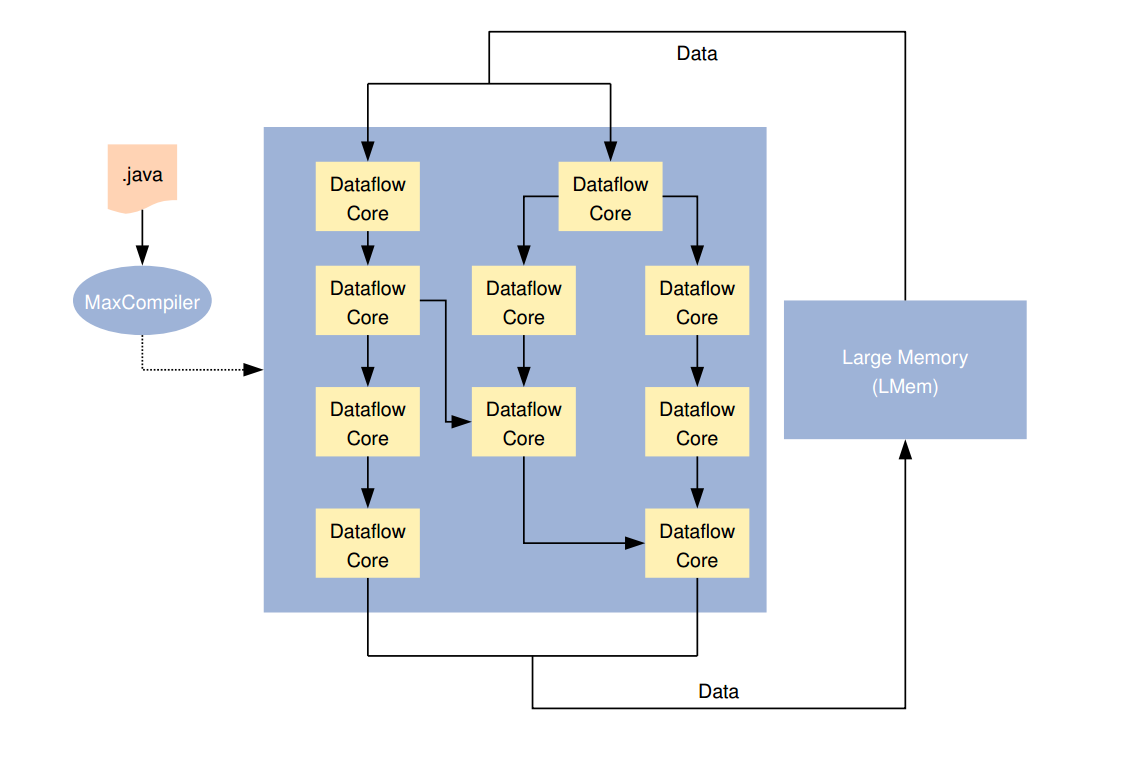
\includegraphics[scale=0.5]{images/DFE}
	\caption{Dataflow model\cite{maxeler}}
\end{figure}

\noindent Figure shows the DFE architecture. The flow of data in the DFE is directed by a manager. The Fast Memory (FMem) lies on the processing chip itself and has a high access bandwidth for fast execution within the chip. The large memory (LMem) lies outside then chip and is able to store a large amount of data \cite{dataflow}. 

\begin{figure}[H]
	\centering
	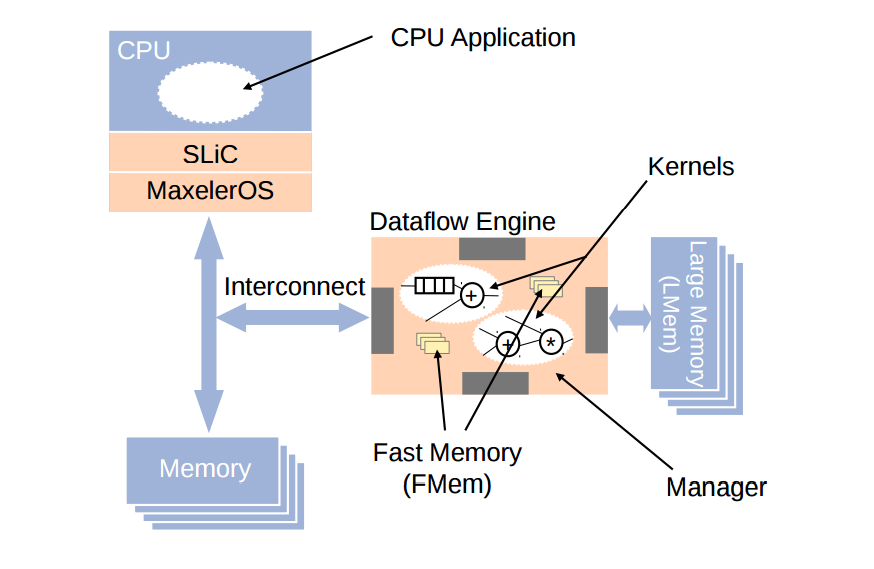
\includegraphics[scale=0.5]{images/DFEarchitecture}
	\caption{Dataflow model\cite{maxeler}}
\end{figure}



\subsection{Simulation}
There are three types of experiments. The most obvious of which is \textit{in vivo} experiments which is to run an actual application on a real hardware platform. However, there may not be a platform available for experimentation purposes. Moreover, if there is a platform available for experimentation, experiments can only be conducted for the platform configurations that are allowed by the platform. This limits the range of experimental scenarios. Another type of experimentation is \textit{in vitro} experiments, which is to run real applications on synthetic platforms. This approach takes care of the issues with running the experiments on a real platform. However, both these methods can be time consuming. The third approach is \textit{in silico}, which is using simulation. This involves running prototypes of applications on system's models and is typically less labour intensive and less costly in terms of hardware resources. Also, it can enable fully repeatable and configurable experiments providing a wide range of experimental scenarios.
\\\\
There are however, a two main concerns with simulation. These are accuracy and scalability. Accuracy is a measure of the validity of the simulation results and scalability refers to how fast and efficient it is with its memory.  Scalability is easily measured whereas for many simulators, accuracy can be largely unknown because they have not been sufficiently validated. This is because it is difficult to evaluate the accuracy. There is a well known trade-off between these two concerns. For example, having a simple simulation model based on mathematical equations would be less demanding in terms of computational power and memory than a complex event-driven model but it may be less accurate. 

\subsection{SimGrid}

SimGrid has been chosen as the simulator for this project. This subsection summarises part of the content from this paper\cite{simulation}, providing a description of SimGrid and the primary motivation of this simulator.
\\\\
\textbf{Design}

\begin{figure}[H]
	\centering
	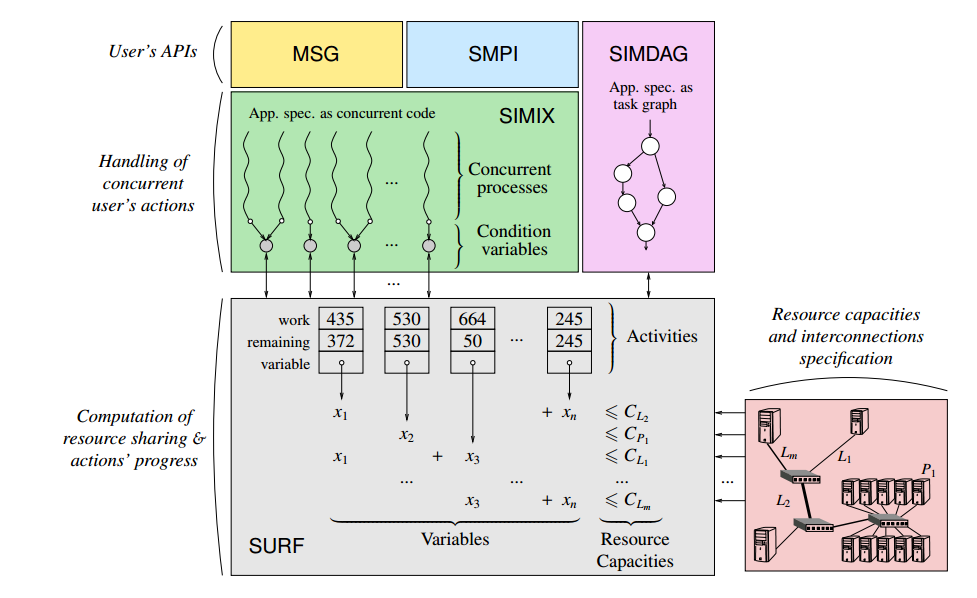
\includegraphics[scale=0.7]{images/simgrid}
	\caption{SimGrid design and internals\cite{simulation}}
\end{figure}

\noindent Figure shows the design and internals of SimGrid.There are three Application Programming Interfaces(APIs) in SimGrid: SMPI, MSG and SimDAG. Users are able to define simulated applications as concurrent processes through the MSG API. The MSG calls are used to simulate the computation and communication of the tasks described by the user. The SMPI API automatically generates processes from an existing application that uses the Message Passing Interface(MPI)  standard. SIMIX is a kernel and handles process control and synchronization. The SIMIX box in the middle shows the concurrent processes executed by the SMPI and MSG simulations. The concurrent processes synchronize on a set of conditional variables as shown in the figure. SimDAG allows the user to specify a Direct Acyclic Graph(DAG) of tasks. It does not use concurrent processes but it is useful for simulating computational tasks which communicate in a non-cyclic manner with dependencies.
\\\\
A simulation has to have simulated hardware resources in order to perform the computational and communication activities. The SURF component in the bottom left of Figure simulates the hardware resources which perform the computation and communication of the simulated tasks. Each task has a total amount of work to complete and the remaining amount of work represented by number of CPU cycles for compute tasks or number of bytes for transfer tasks.
\\\\
SimGrid allows the user to model compute resources by simply giving it a number representing the compute speed. Task execution times are then computed by dividing the size of the task by the compute speed. This compute speed can be determined for simulated resources by obtaining results from their corresponding real world resources.
\\\\



\subsection{Other Simulators}
\textbf{SimMatrix}
\\\\
The SimMatrix mini-section below is mostly obtained from \cite{simmatrix} and provides information about SimMatrix and what this simulator aims to achieve with its design and architecture.
\\\\
Exascale computing is computing that may have up to millions of nodes and billions of threads of execution. The four main challenges of exascale computing are energy and power; memory and storage; concurrency and locality; resiliency. Many-Task Computing (MTC) was introduced with the idea of accomplishing many tasks using a large number of computing resources over a short period of time. It can potentially address three of four of these challenges except the power and energy problem. Its asynchronous nature provides good resiliency as it allows easy task level checkpointing and failures only affect tasks running on failed nodes. However, scalable storage systems are required to achieve asynchronous inter-process communication and the task management system has to be much more scalable and flexible in order to handle the large number of tasks in MTC applications. SimMatrix is a light-weight and scalable discrete-event simulator. It supports both centralized and distributed scheduling.

\begin{figure}[H]
	\centering
	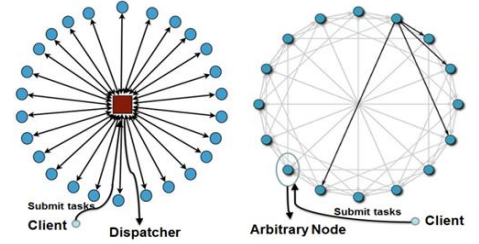
\includegraphics[scale=1.1]{images/scheduling}
	\caption{Centralized(left) and distributed(right) scheduling\cite{simmatrix}}
\end{figure}

\noindent SimMatrix was compared to SimGrid terms of resources required per task. SimMatrix could potentially work better for large systems with large number of nodes and tasks. However, it may not be as versatile as SimGrid as its primary focus is on scalability. Thus, SimGrid was chosen SimMatrix because the project's main aim is to be able to model heterogeneous systems. 

\section{Design}

First an application has to be defined. Then the application is run on a few different platform configurations with a range of input sizes to obtain some data points. These data points are then used to obtain a function through basic fitting which will be used in the simulation model. For each platform configuration, each experiment involves choosing a specific workload size and running the application to obtain the throughput of the platform. Then a scatter plot of the throughput of the platform against the workload size is made and a fitting function is obtained from the scatter plot. This function will then be used to model the platform. 

\section{Modelling Heterogeneous Systems}

In this section, I explain how I derived the performance models for the AdPredictor application running on multicore CPUs for different number of cores and multiDFE systems for different number of DFEs. In these experiments, the AdPrediction application is viewed as a black box, where I only look at the size of the workload going in and the throughput of the application. Then, I explain how I used these performance models to create simulated resources in SimGrid.

\subsection{Multicore CPU}
Dr. Figuiredo provided me with an application that allows the user to specify the workload of the application and the number of CPU cores used for the application and calculates the time taken to run the application and the throughput. By using the method described above, I was able to create a simulation model for a multicore CPU for this application.
\\\\
I used the multicore CPU in the maxnode2 to obtain data for one to ten CPU cores. For each number $n$ of CPU cores, a set of 20 data points were obtained. MATLAB was used to generate the scatter plots for these data sets and generate a fitting function that models the performance for different number of CPU cores.

\begin{figure}[H]
	\hspace*{-2.8cm}  
	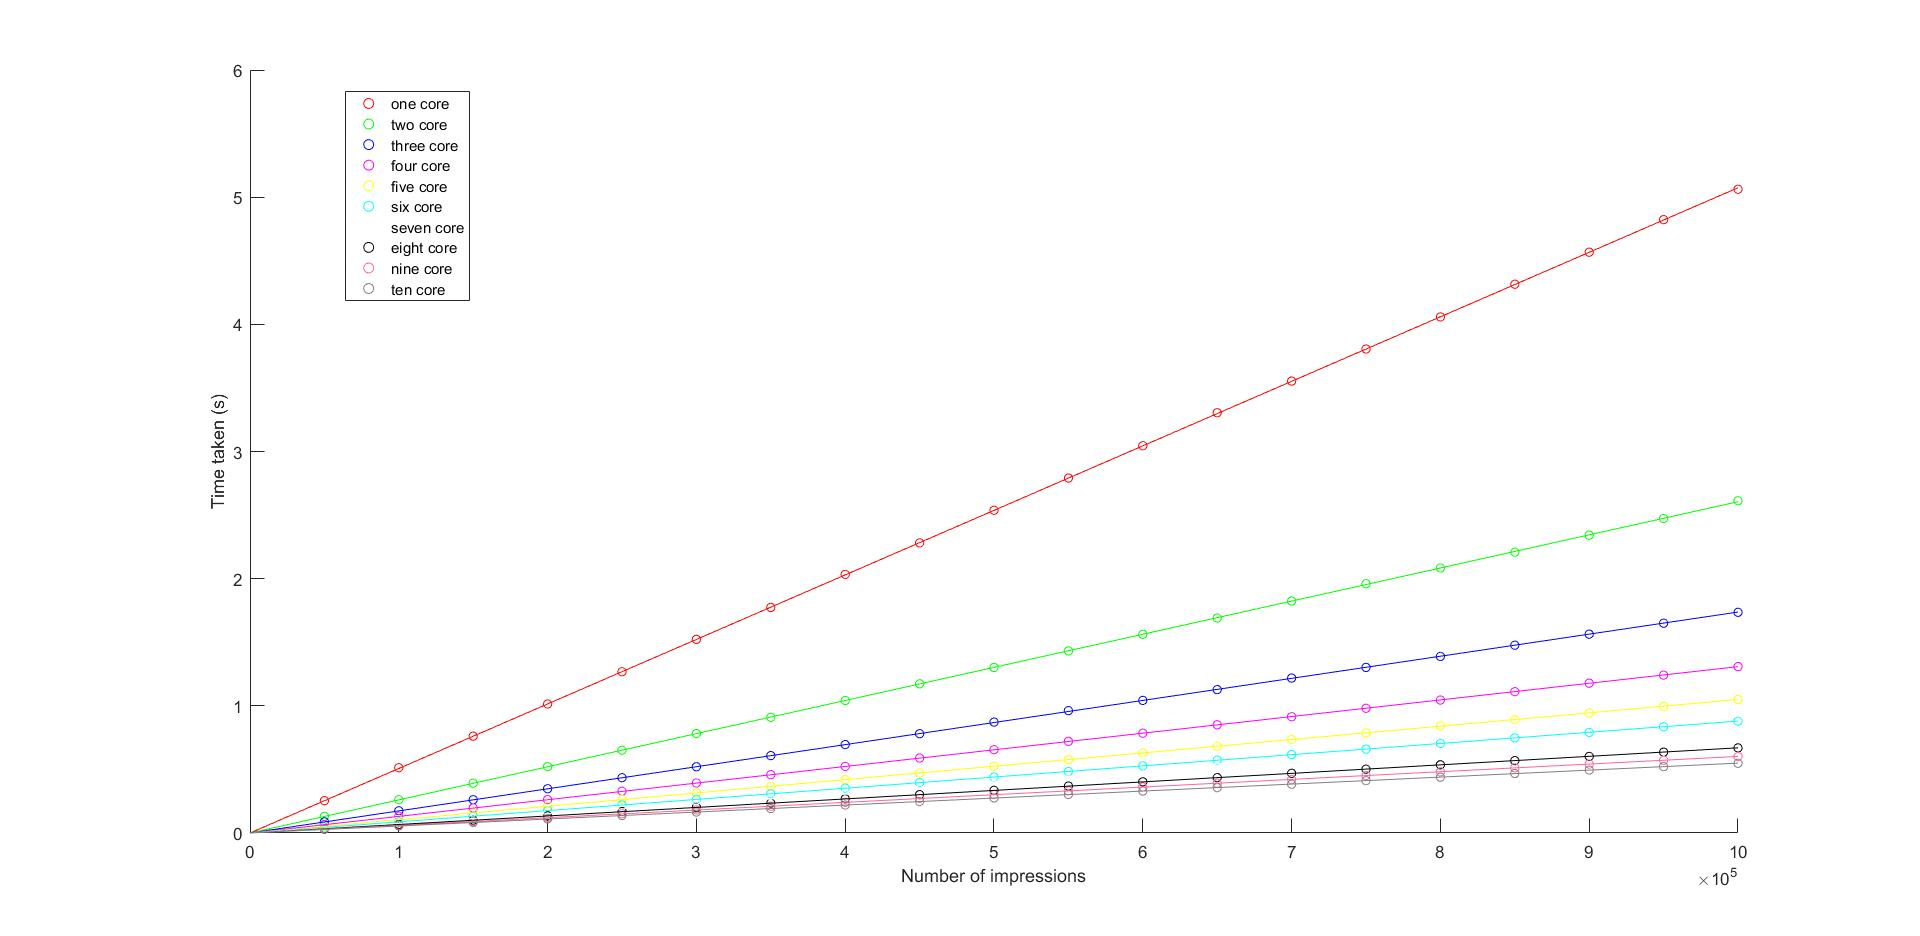
\includegraphics[scale=0.3]{images/impressions_time}
	\caption{AdpPredictor CPU}
\end{figure}

\noindent Figure 5 shows the data points obtained for number of impressions against time for one to four CPU cores. Below are the four equations obtained from the by fitting these points.

\begin{equation}
y = 5.074\times 10^{-6}x
\end{equation}

\begin{equation}
y = 2.605\times 10^{-6}x
\end{equation}

\begin{equation}
y = 1.738\times 10^{-6}x
\end{equation}

\begin{equation}
y = 1.308\times 10^{-6}x
\end{equation}

\begin{equation}
y = 1.050\times 10^{-6}x
\end{equation}

\begin{equation}
y = 8.801\times 10^{-6}x
\end{equation}

\begin{equation}
y = 7.614\times 10^{-6}x
\end{equation}

\begin{equation}
y = 6.699\times 10^{-6}x
\end{equation}

\begin{equation}
y = 6.023\times 10^{-6}x
\end{equation}

\begin{equation}
y = 5.494\times 10^{-6}x
\end{equation}

\noindent Equation $(i)$ represents the fitted curve for $i$ cores for $0 \leq i \leq 4$ The reciprocal of the gradient of these linear curves can be used as an estimate of the average throughput of each number of cores in impressions/s. By further experimentation, this can be used to estimate the throughput of any number of cores.
\\\\
\noindent After obtaining the equations, I modelled the multicore CPU using the MSG API in SimGrid. Using the reciprocal of the gradient of the one core CPU plot from Figure 5 as the power of one CPU core. Figure 6 shows the same plot as Figure 5 for the SimGrid simulation.

\begin{figure}[H]
	\hspace*{-2.8cm}  
	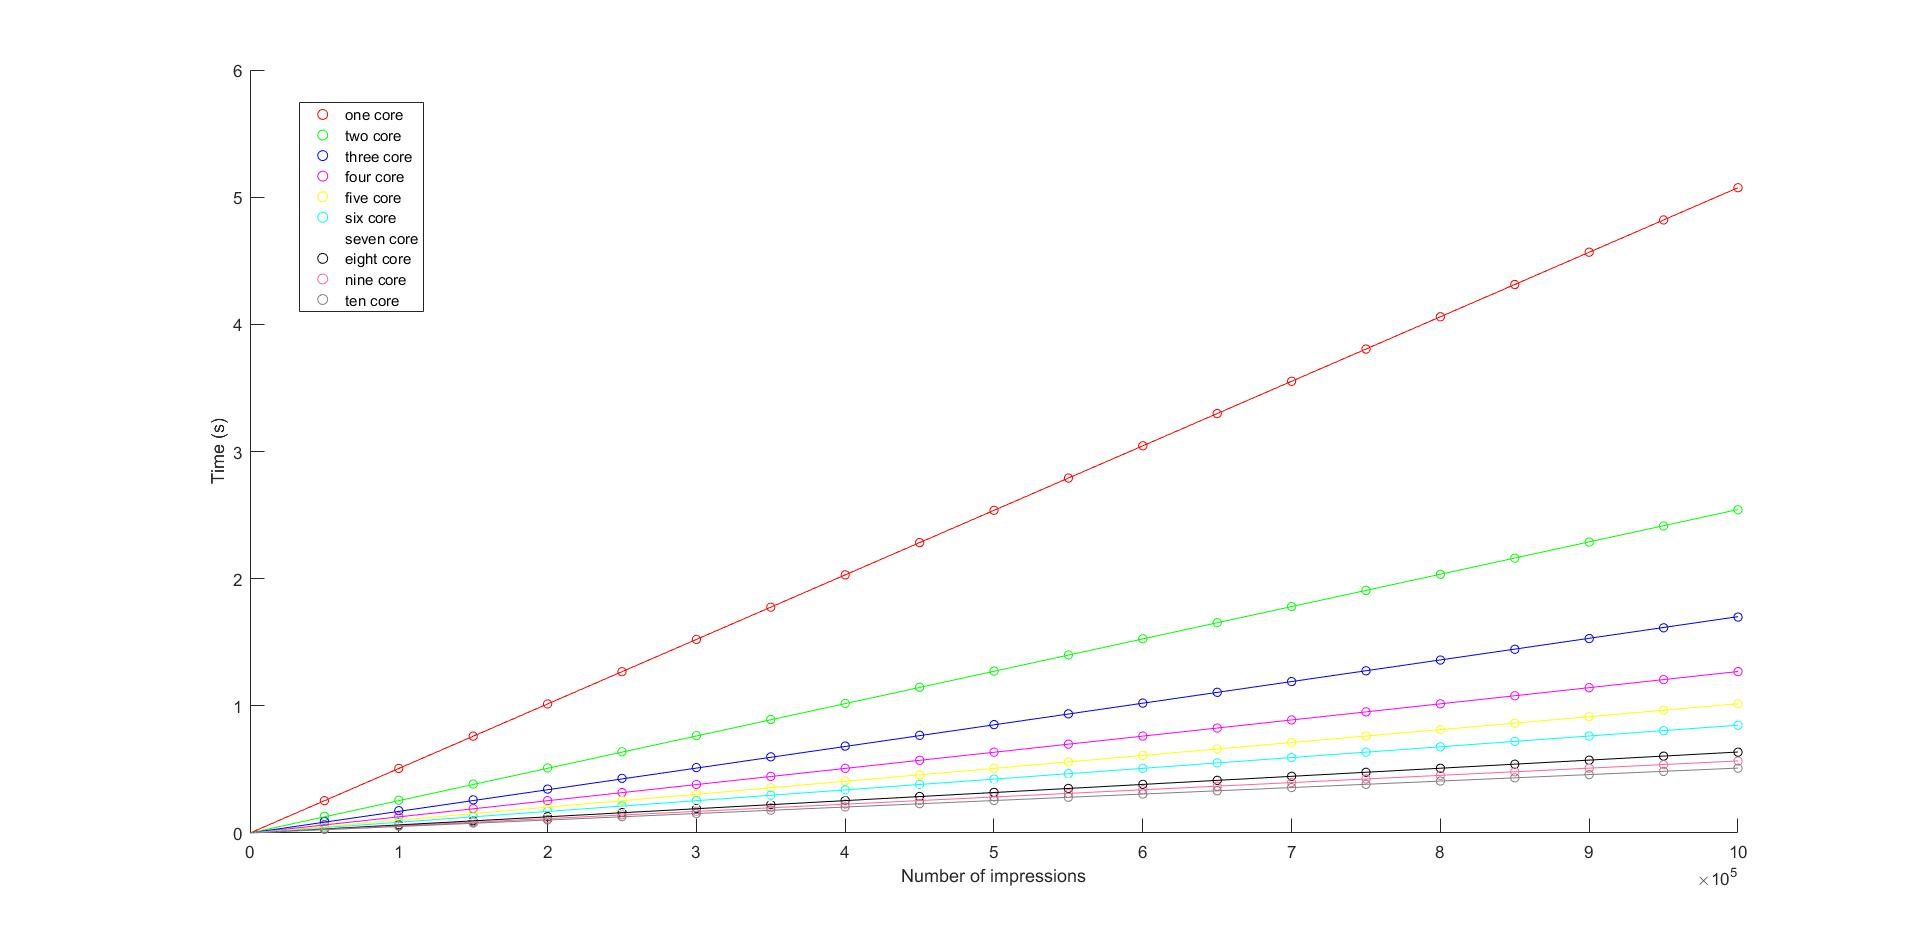
\includegraphics[scale=0.3]{images/multicore_sim}
	\caption{SimGrid simulation plot}
\end{figure}

\noindent Below are the corresponding equations.

\begin{equation}
y = 5.074\times 10^{-6}x
\end{equation}

\begin{equation}
y = 2.605\times 10^{-6}x
\end{equation}

\begin{equation}
y = 1.738\times 10^{-6}x
\end{equation}

\begin{equation}
y = 1.308\times 10^{-6}x
\end{equation}

\begin{equation}
y = 1.050\times 10^{-6}x
\end{equation}

\begin{equation}
y = 8.801\times 10^{-6}x
\end{equation}

\begin{equation}
y = 7.614\times 10^{-6}x
\end{equation}

\begin{equation}
y = 6.699\times 10^{-6}x
\end{equation}

\begin{equation}
y = 6.023\times 10^{-6}x
\end{equation}

\begin{equation}
y = 5.494\times 10^{-6}x
\end{equation}

\noindent The results from the simulation are then compared to the results from running the actual application on real hardware to see if the simulation was accurate. Figure shows the comparison between the two plots from Figures 5 and 6.

\begin{figure}[H]
	\hspace*{-2.8cm}  
	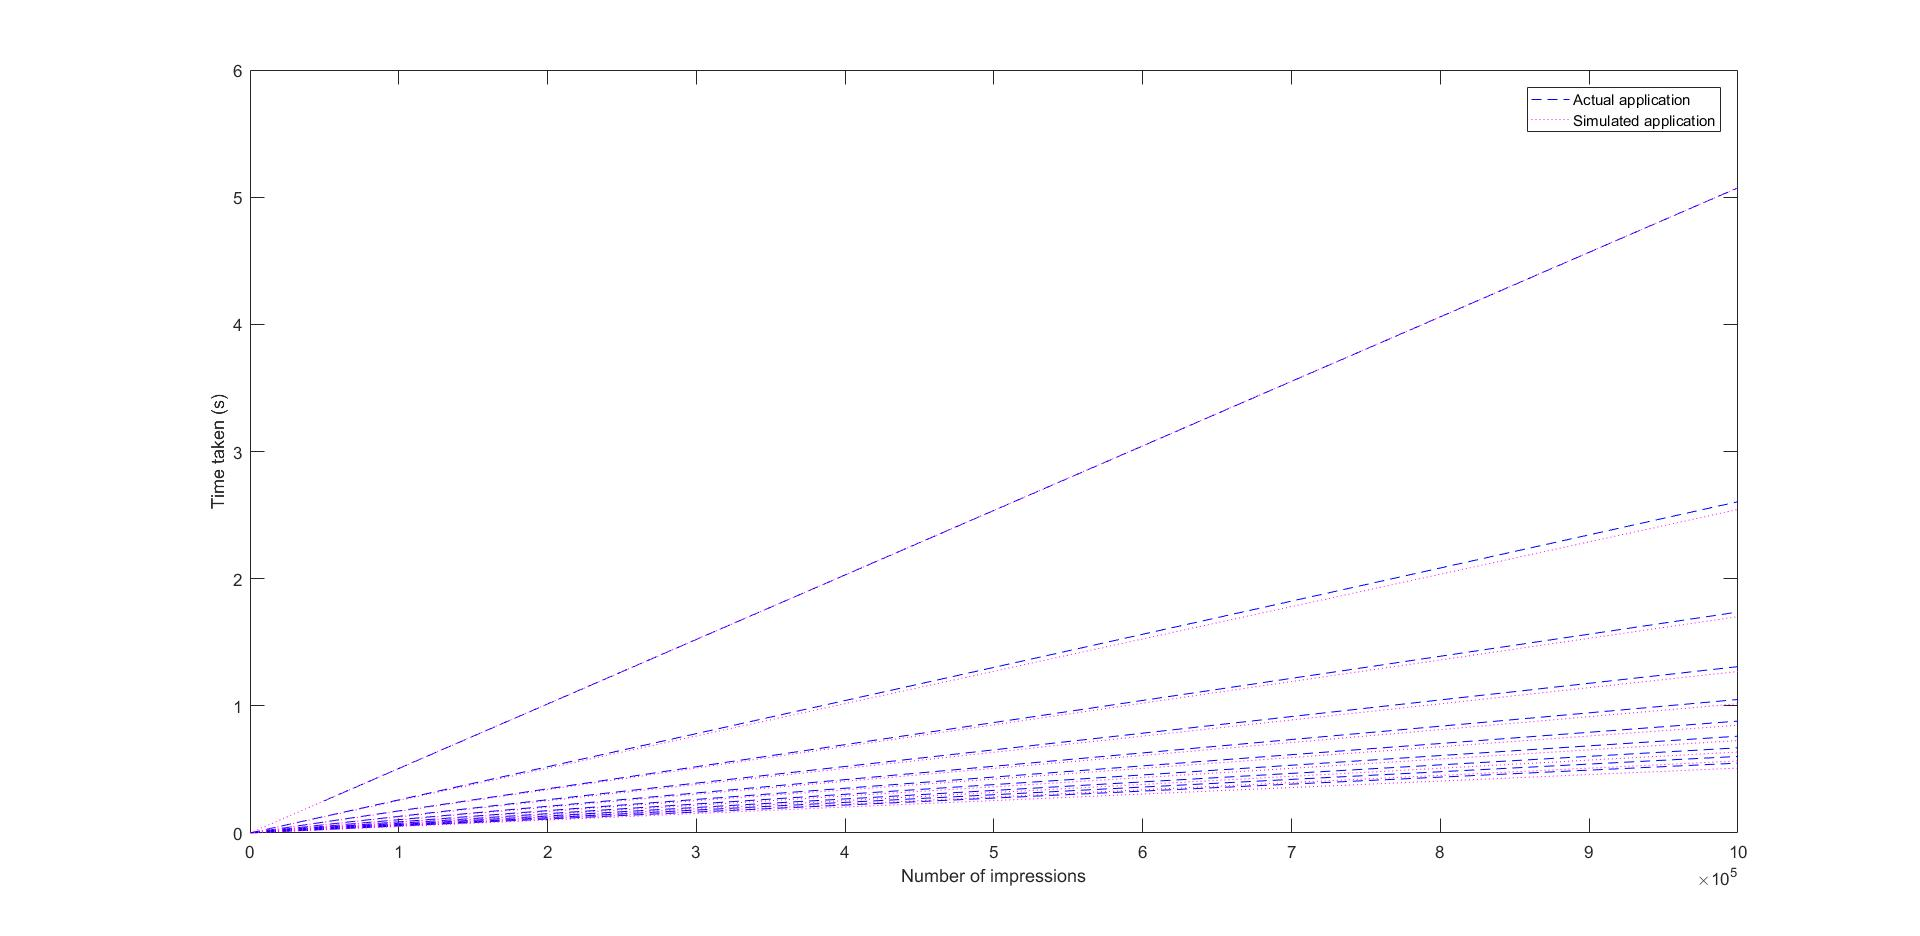
\includegraphics[scale=0.3]{images/multicore_compare}
	\caption{SimGrid simulation plot}
\end{figure}

\noindent The results for the one core to three cores plots show that the simulation quite accurately models the real application for these cases. However, there is a slight error rate in the four cores case. This may imply that the error rate may increase as the number of cores intended to model increases but my computer does not have the resources to further investigate these cases. 
\\\\
\noindent Another experiment that was done was to plot the log of number of impressions against the throughput of each number of cores to observe the changes in throughput from a small workload to a large workload. Figure 8 shows the performance model for each number of cores.

\begin{figure}[H]
	\hspace*{-2.8cm}  
	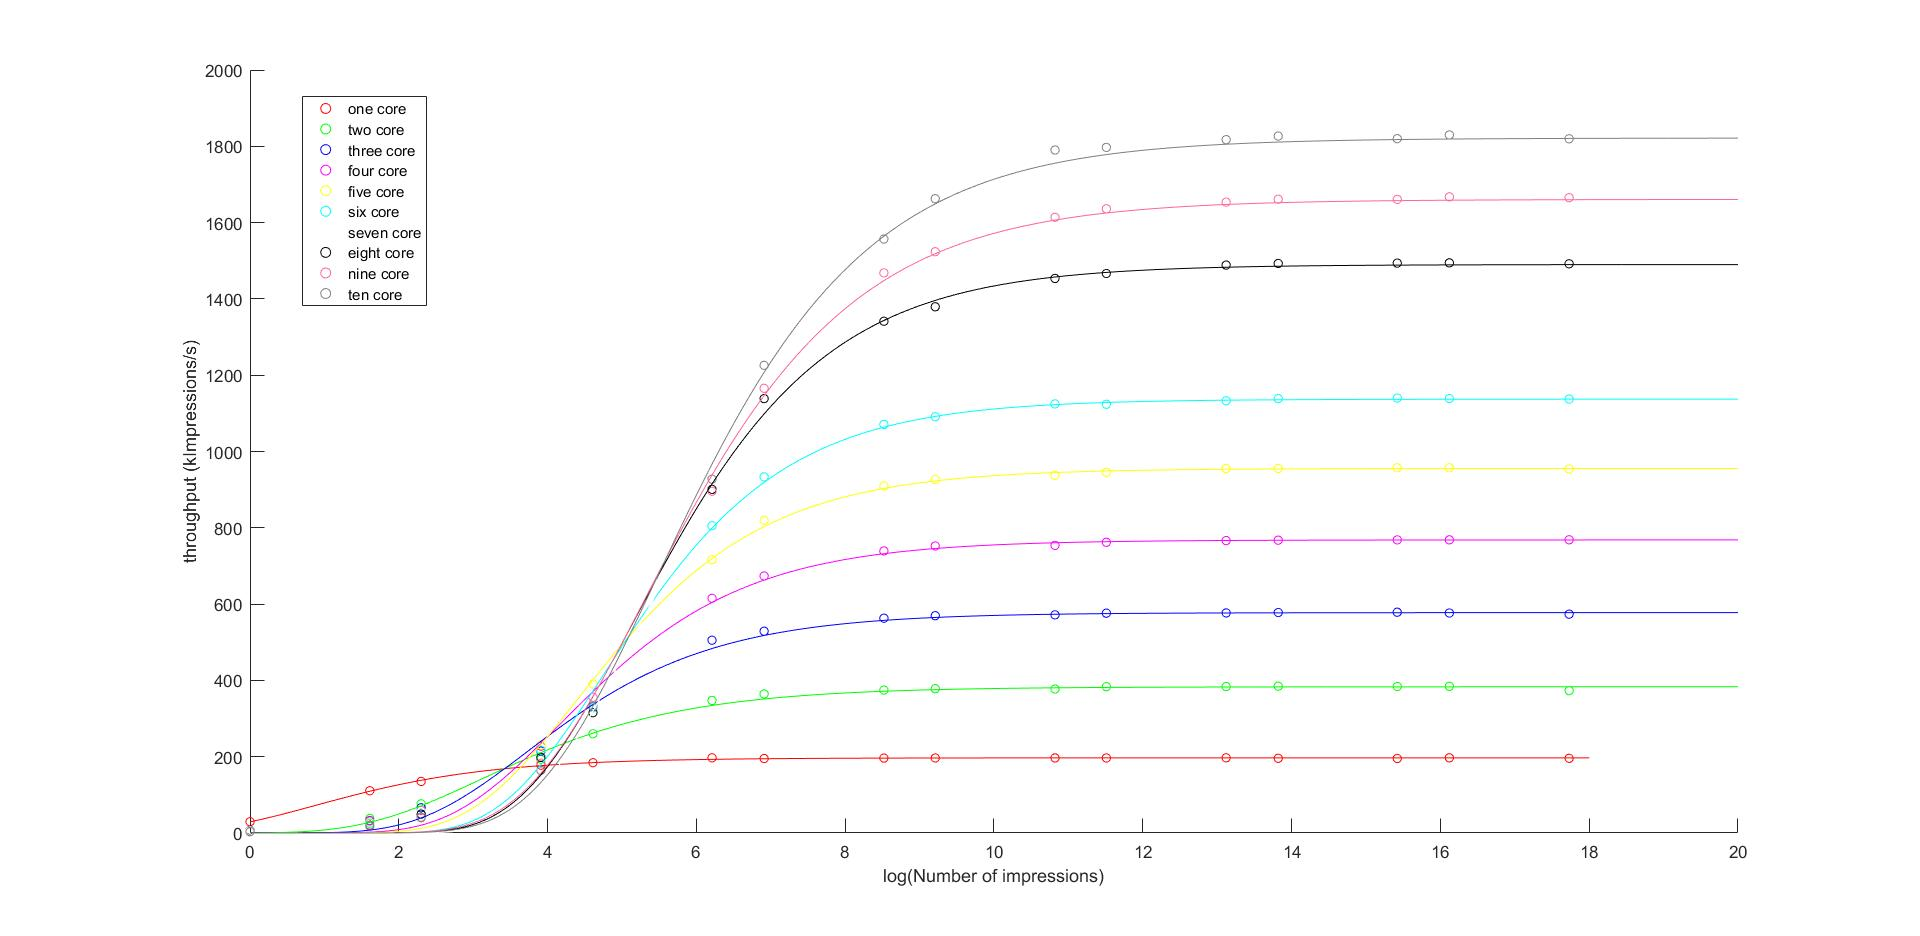
\includegraphics[scale=0.3]{images/logimpressions_throughput}
	\caption{Throughput against log(number of impressions)}
\end{figure}

\noindent The results show that for a smaller workload, using less cores may result in a higher throughput. This experiment shows the performance for each number of cores for low workloads and high workloads, providing a more accurate model than the first experiment. The data points from this experiment appear to have the shape of the Gompertz function\cite{Gompertz}, which is of the form $ae^{-be^{-cx}}$.  For small workloads, the throughput start increasing slowly. Then it increases faster until it converges to its maximum value and plateaus. The curves above are obtained by using MATLAB\cite{MATLAB} to fit the points using this equation and calculating the corresponding values for the coefficients $a$, $b$ and $c$. Below are the equations obtained for each number of cores.

\begin{equation}
y = 197e^{-1.906e^{-0.7301x}}
\end{equation}

\begin{equation}
y = 383.3e^{-7.347e^{-0.6417x}}
\end{equation}

\begin{equation}
y = 577.6e^{-13.23e^{-0.694x}}
\end{equation}

\begin{equation}
y = 768.2e^{-17.92e^{-0.6947x}}
\end{equation}

\begin{equation}
y = 955.5e^{-21.78e^{-0.6992x}}
\end{equation}

\begin{equation}
y = 1137e^{-30.92e^{-0.7205x}}
\end{equation}

\begin{equation}
y = 1318e^{-46.81e^{-0.7588x}}
\end{equation}

\begin{equation}
y = 1490e^{-31.39e^{-0.6706x}}
\end{equation}

\begin{equation}
y = 1661e^{-26.38e^{-0.6192x}}
\end{equation}

\begin{equation}
y = 1822e^{-29.27e^{-0.6172x}}
\end{equation}

\noindent Using these values for $a$, $b$ and $c$, it is possible to predict the performance models for a larger number of CPU cores. Furthermore, it is simpler to model a multicore CPU as a single compute node with a power that is calculated using the equation for the corresponding number of cores as opposed to modelling it as multiple compute nodes where the tasks have to be assigned to each one individually.

\begin{figure}[H]
	\hspace{-2.8cm}
	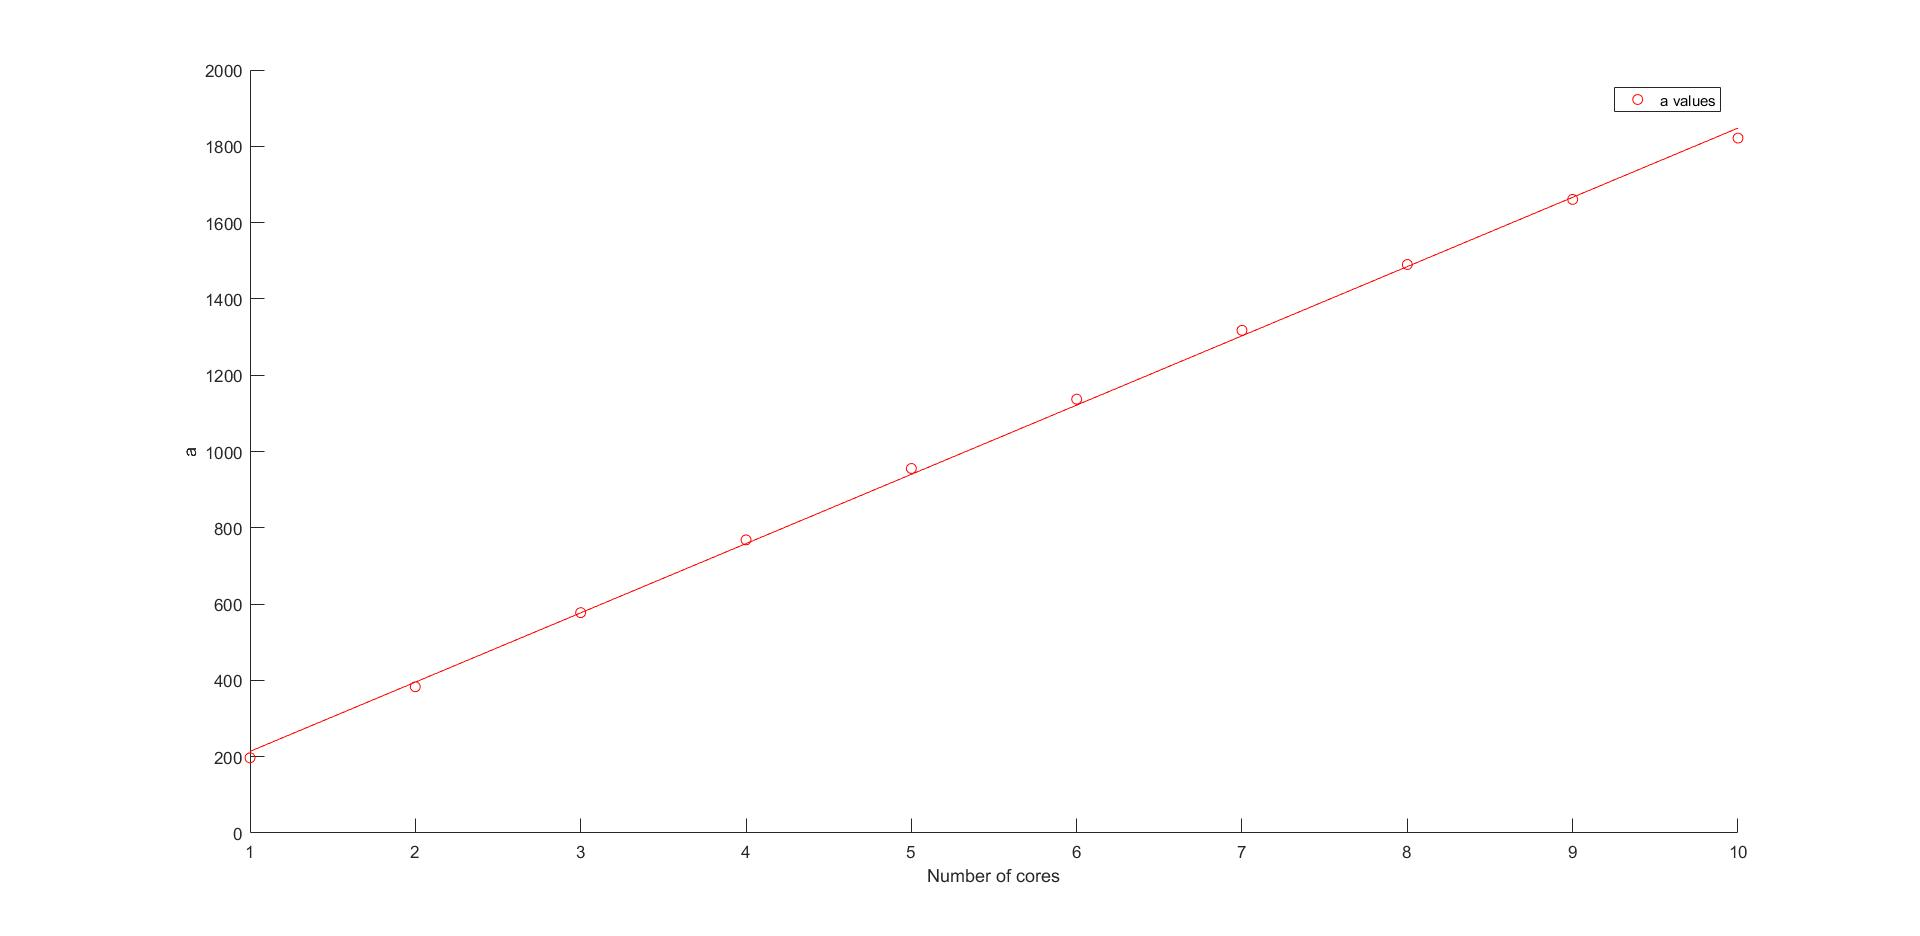
\includegraphics[scale=0.3]{images/multicore_a}
	\caption{$a$ against Number of cores}
\end{figure}

\noindent Figure 9 shows the plot for $a$ values, which appears to increase linearly with the number of cores. Hence, a linear function was used to fit this data.

\begin{equation}
y = 181.5x + 32.38
\end{equation}

\noindent The $a$ coefficient of the Gompertz function represents the value that the curve converges to. In this case, it should be the maximum throughput of the corresponding number of cores. I determined this value by taking the average of the last 6 values for each dataset. By specifying this in MATLAB's fit function, it helped MATLAB to produce a better fit for the dataset.

\begin{figure}[H]
	\hspace{-2.8cm}
	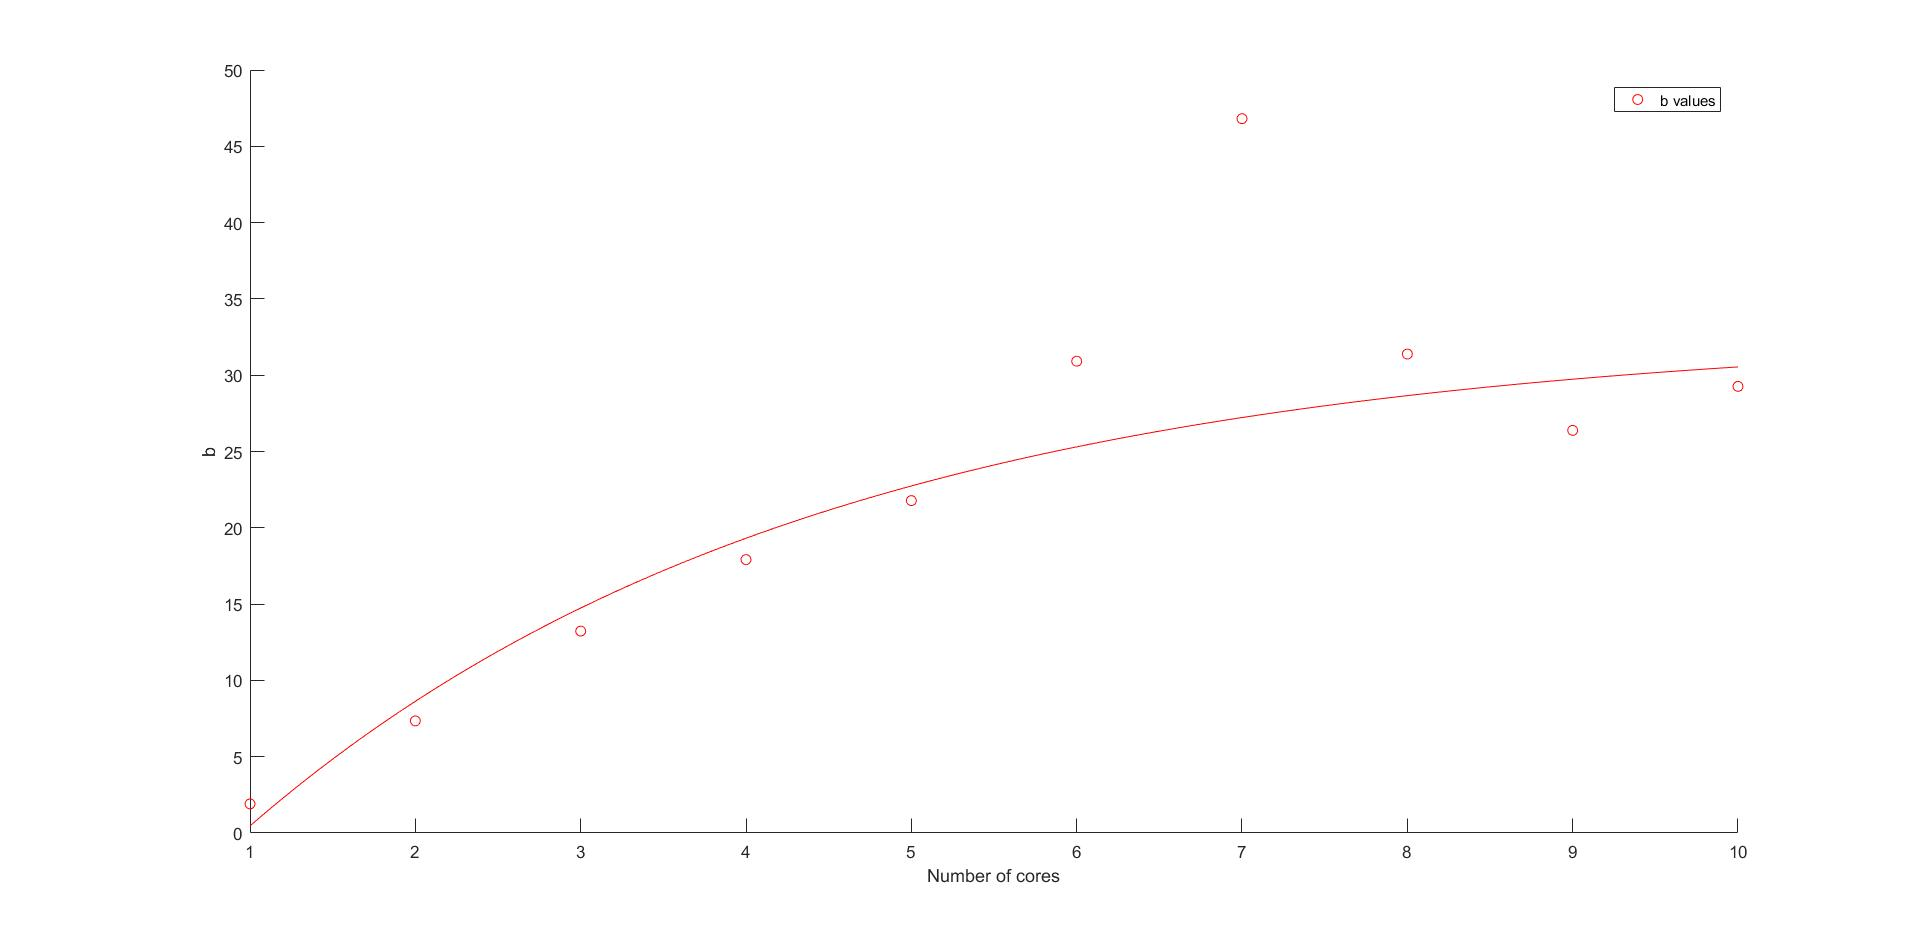
\includegraphics[scale=0.3]{images/multicore_b}
	\caption{$b$ against Number of cores}
\end{figure}

\noindent Figure 10 shows the plot for $b$ values, which seem to converge to some value as the number of cores increases. Below is the equation used to fit the data.

\begin{equation}
y = 43.38(1-e^{-0.2896x})-10.44
\end{equation}

\noindent The $b$ coefficient represents the horizontal shift of the curve which seems to be converging. As you can observe in Figure 8, as the number of cores increases, the mid point of the curve moves from left to right but the shift gradually decreases, hence, I chose to use the equation in the form $a(1-e^{-bx})-c$.

\begin{figure}[H]
	\hspace{-2.8cm}
	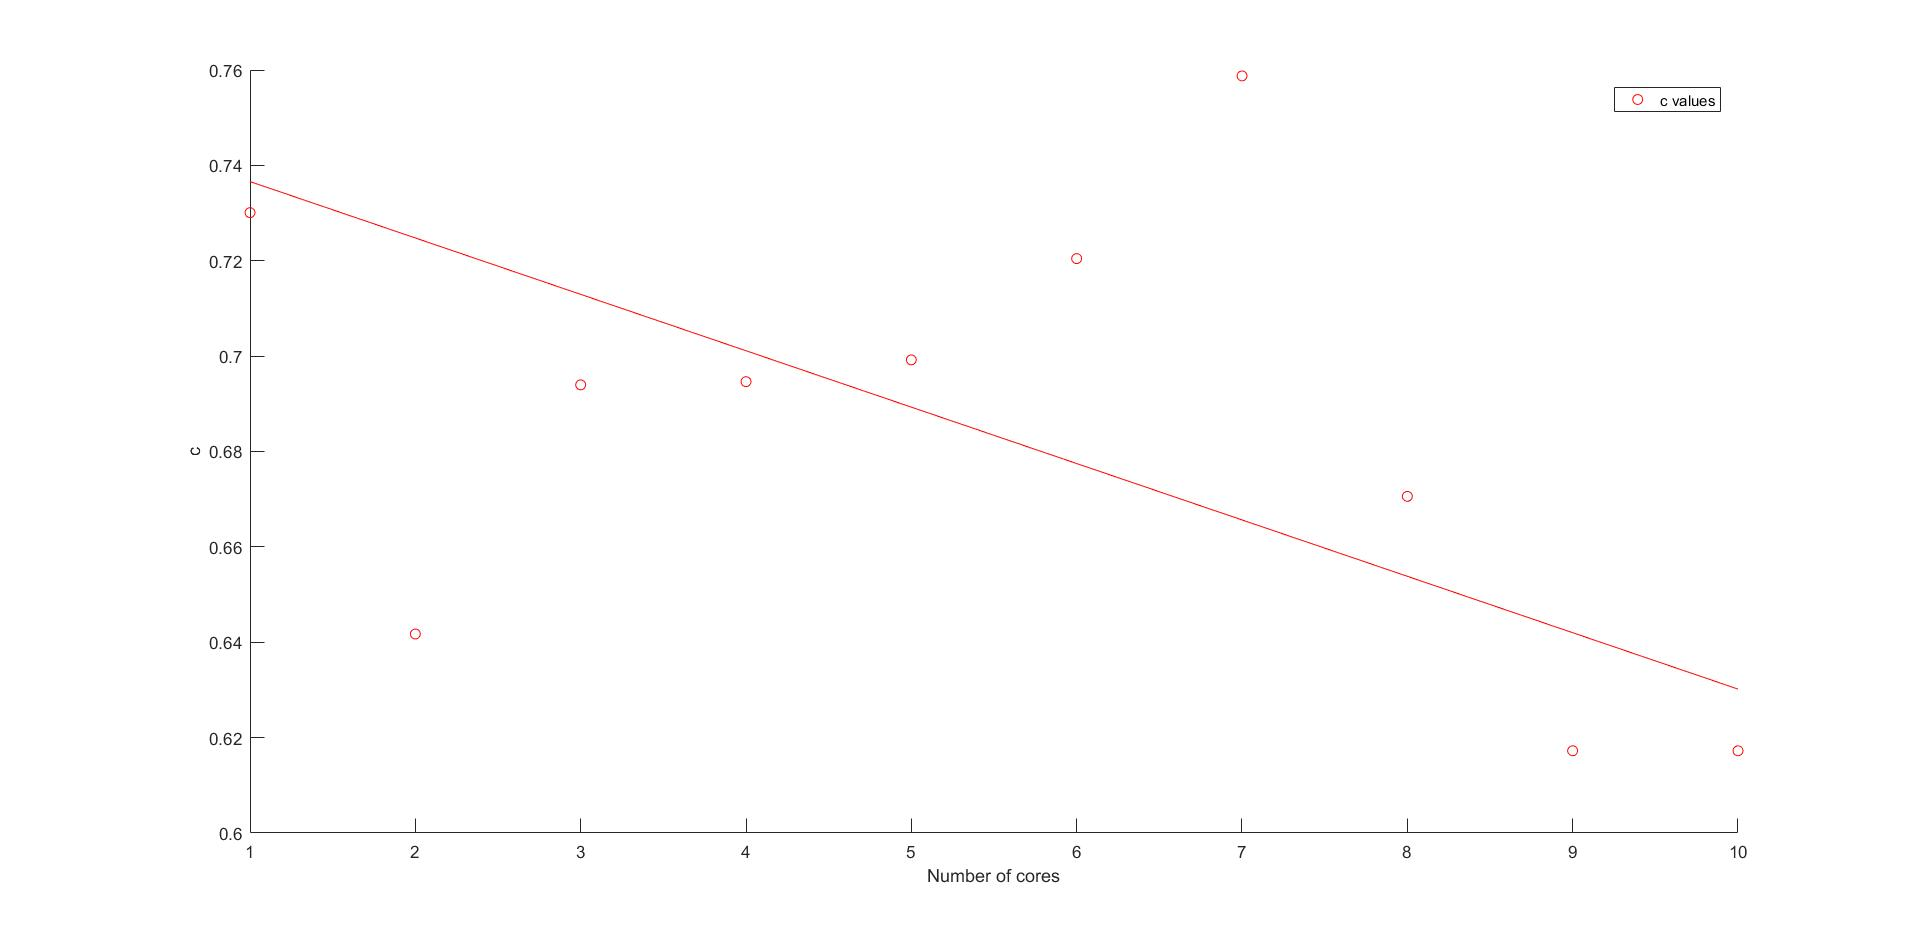
\includegraphics[scale=0.3]{images/multicore_c}
	\caption{$c$ against Number of cores}
\end{figure}

\noindent Figure 11 shows the plot for $c$ values. Below is the equation I choose to fit the data points.

\begin{equation}
y=-0.01183x + 0.7484
\end{equation}

\noindent The $c$ coefficient represents the rate of increase of the curve. It was quite difficult to fit the data points for this coefficient as there is no clear pattern as seen in Figure 11. But I think it should be continuously decreasing as a higher number of cores would have a steeper slope in the middle and gentler at the ends. Hence, I decided to use a linear model. However, this may not be entirely accurate, but it should still preserve the information we need about the performance model, that is, which number of cores performs better at a given workload size.

\subsection{MultiDFE}
The same as above was done on multiple DFEs to see if modelling multiDFEs would be different from modelling multicore CPUs.

\begin{figure}[H]
	\hspace{-2.8cm}
	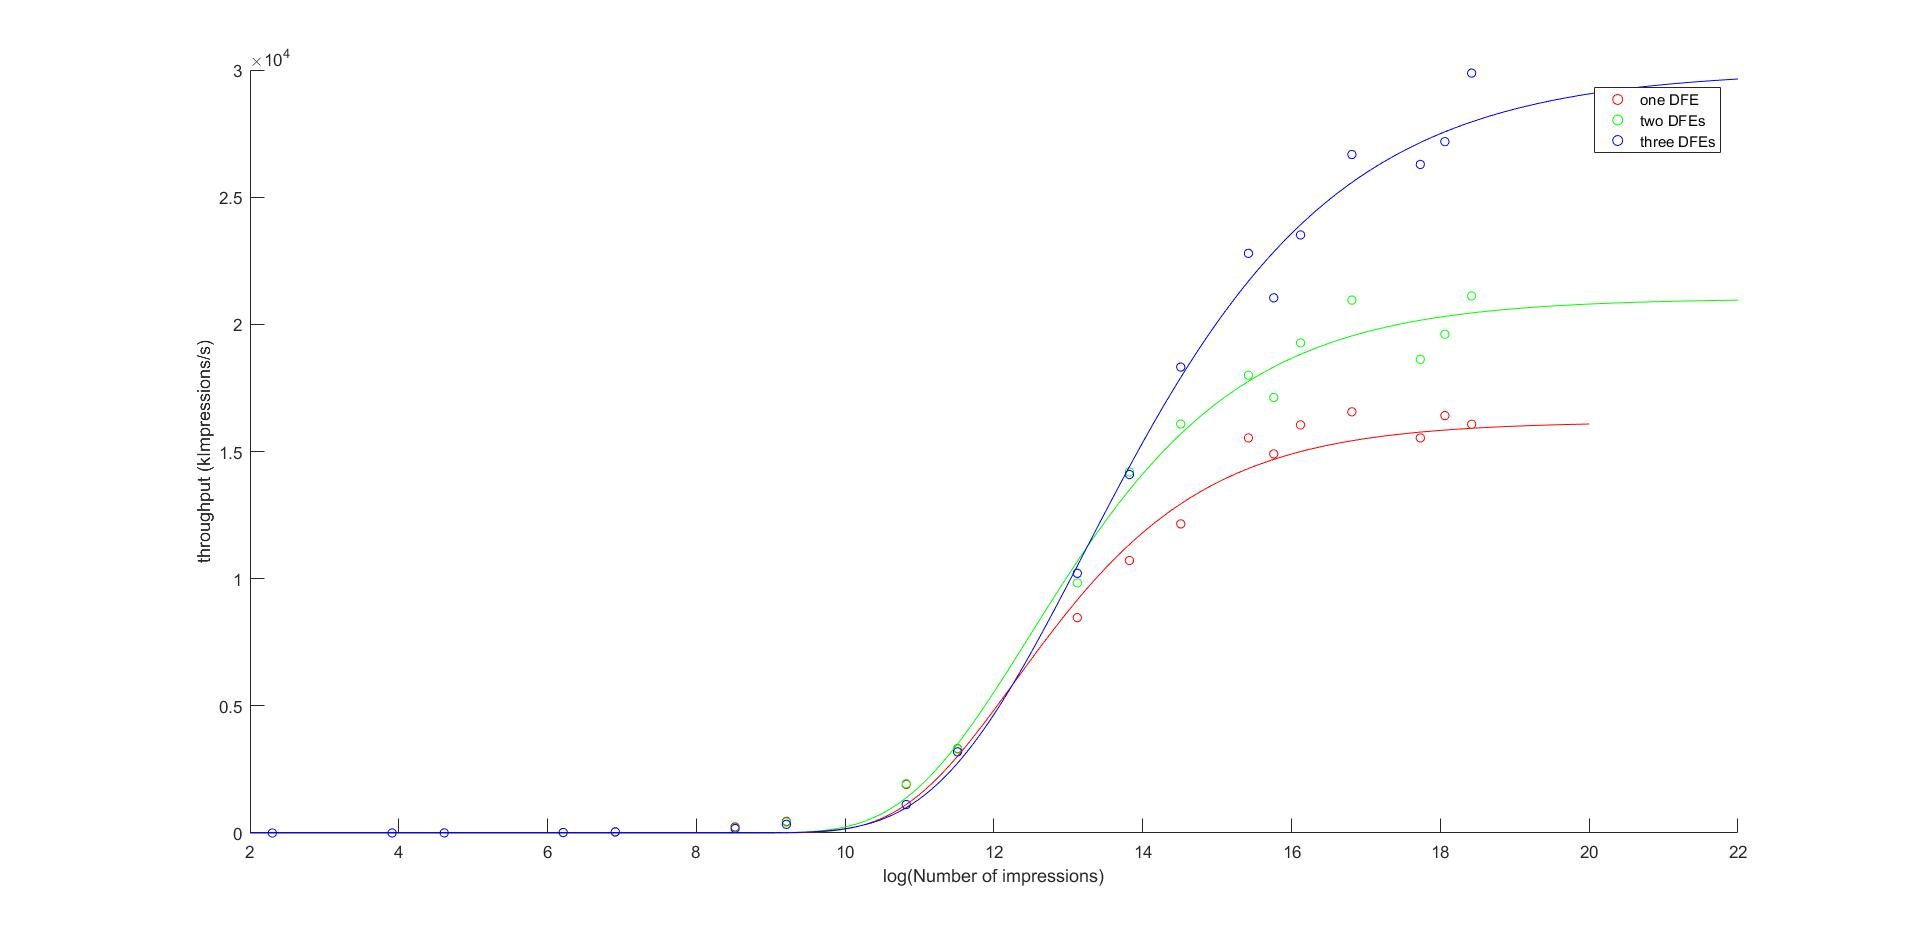
\includegraphics[scale=0.3]{images/multidfe}
	\caption{$a$ against Number of cores}
\end{figure}

\noindent It appears that the plot for multiple DFEs can also be fitted using the Gompertz function. However it seems the maxnode2 platform does not have enough heap memory to perform experiments with a higher workload. As such, I could not provide a workload large enough for each number of DFEs to reach its maximum throughput. Hence, although the maxnode2 has four DFEs, I only plotted the data for one to three DFEs as it may be difficult to model the data for four DFEs without knowing its maximum throughput. Thus, the equations obtained from these performance models may not accurately represent the hardware resources for extremely large workloads. Below are the plots for the $a$, $b$ and $c$ for the DFE curves. 

\begin{figure}[H]
	\hspace{-2.8cm}
	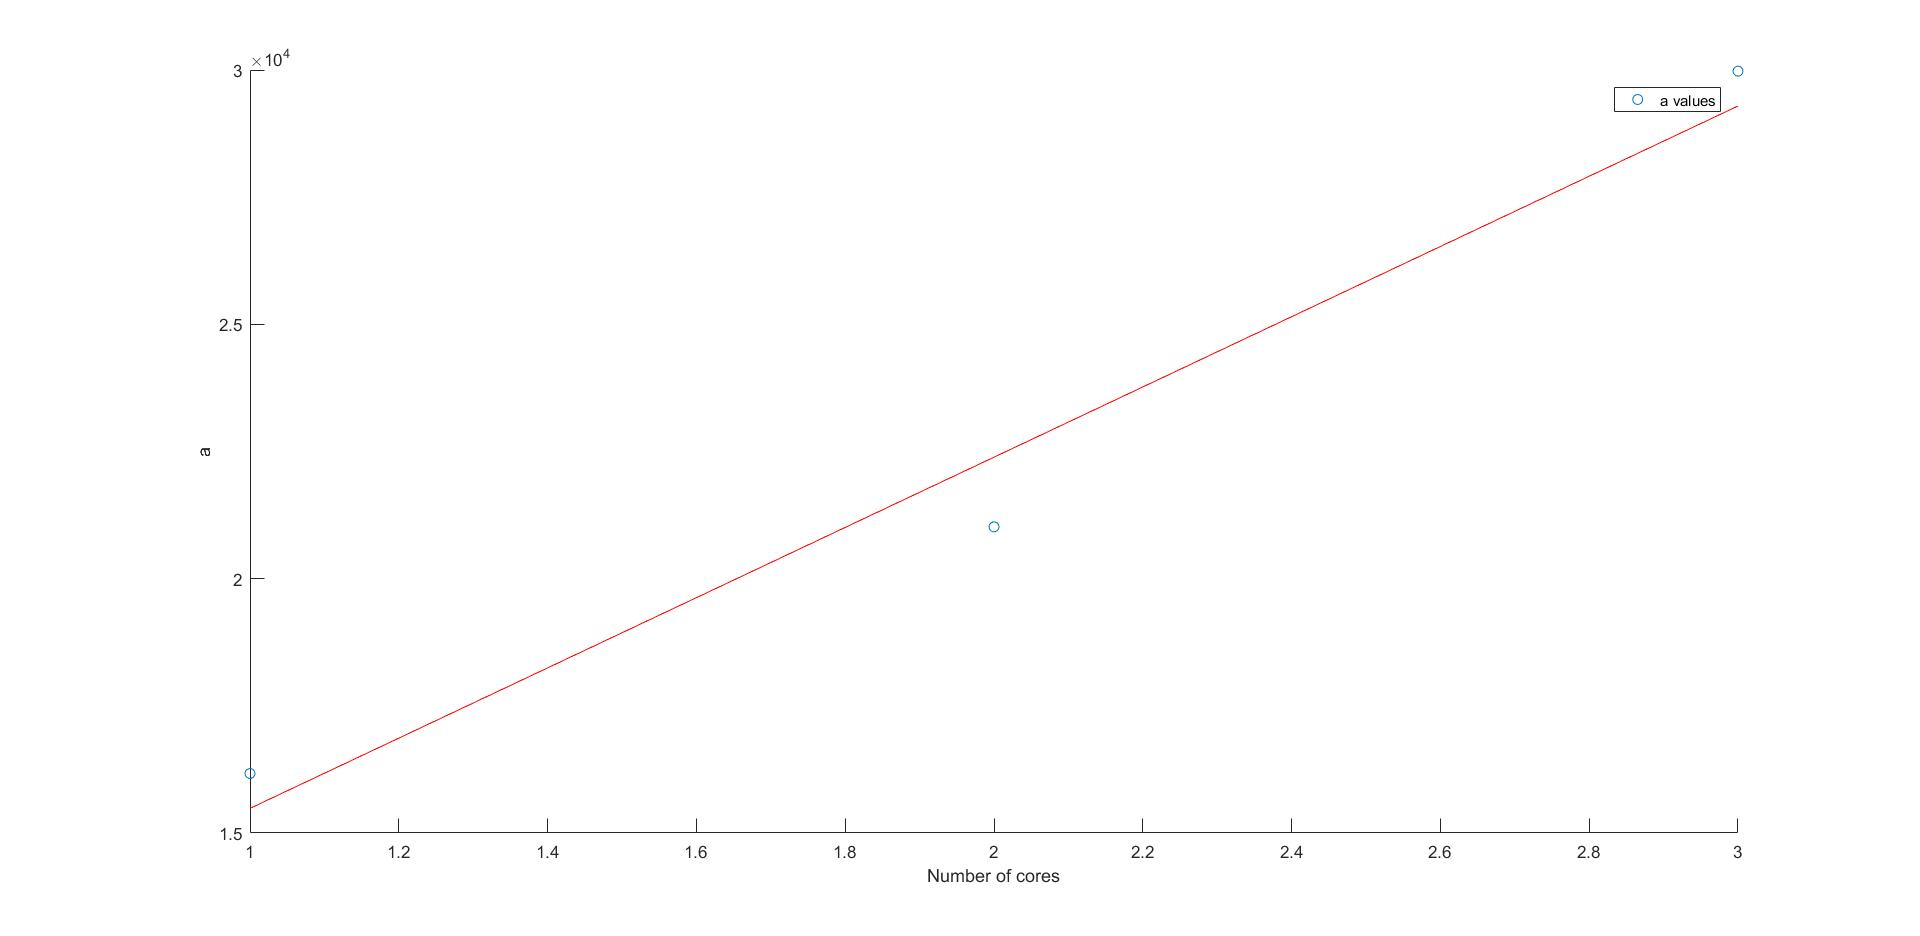
\includegraphics[scale=0.3]{images/dfe_a}
	\caption{$a$ against Number of cores}
\end{figure}

\noindent $a$ appears to increase linearly with the number of DFEs similar to the multicore CPU. Below is the equation used to fit the $a$ values.

\begin{equation}
y=6904x + 8580
\end{equation}

\noindent However, these values may not accurately represent the maximum throughput of the corresponding number of DFEs as seen in Figure 13, the data points have not quite reached a definite convergence point as opposed to what was observed for the multicore CPU case. I would expect that if more experiments can be done, that the increase may be greater.

\begin{figure}[H]
	\hspace{-2.8cm}
	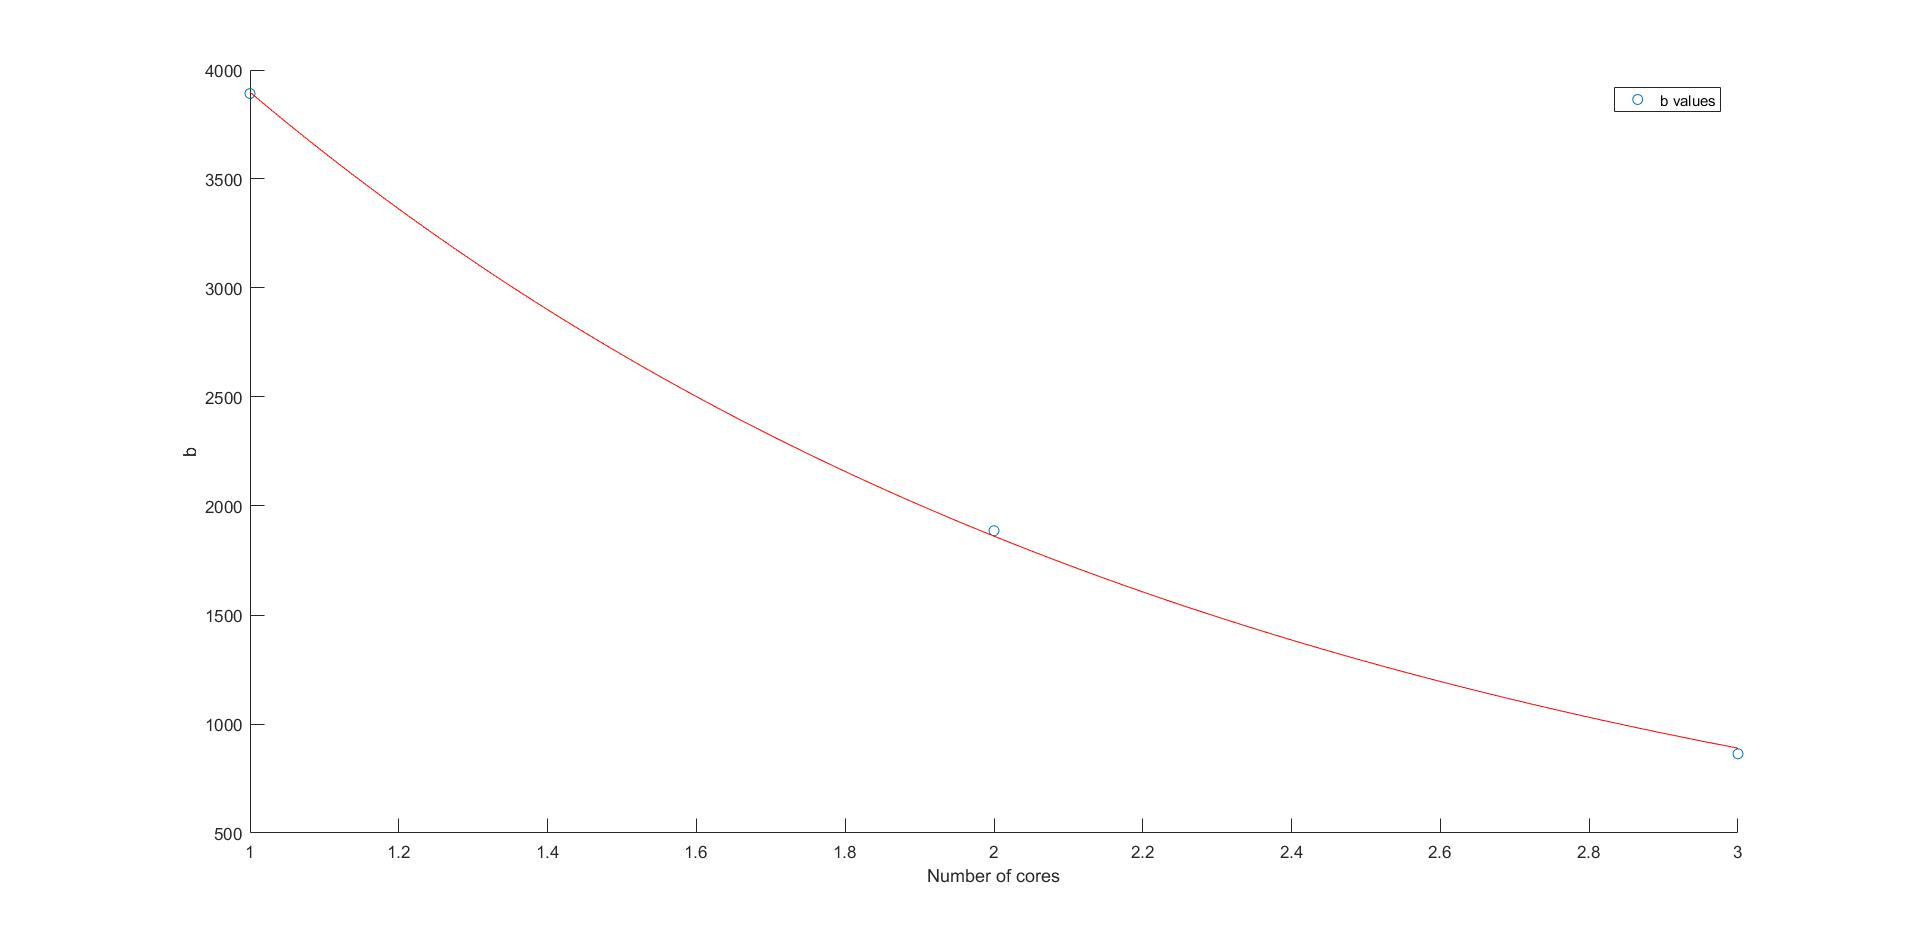
\includegraphics[scale=0.3]{images/dfe_b}
	\caption{$b$ against Number of cores}
\end{figure}

\noindent For the DFEs, the curves are much further to the right since the throughput only starts to increase for a larger workload. Hence, the $b$ coefficient is much larger. Furthermore, the curves appear to be shifting to the left as the number of DFEs increases. Hence, the values for $b$ seems to decrease as the number of DFEs increases as opposed to the values for the multicore CPU as seen in Figure 15.

\begin{equation}
y=8162e^{-0.739x} + 0.000002946
\end{equation}

\noindent The curve equation of the form $ae^{-bx}+c$ was used since the values for $b$ are decreasing and seems to be converging.

\begin{figure}[H]
	\hspace{-2.8cm}
	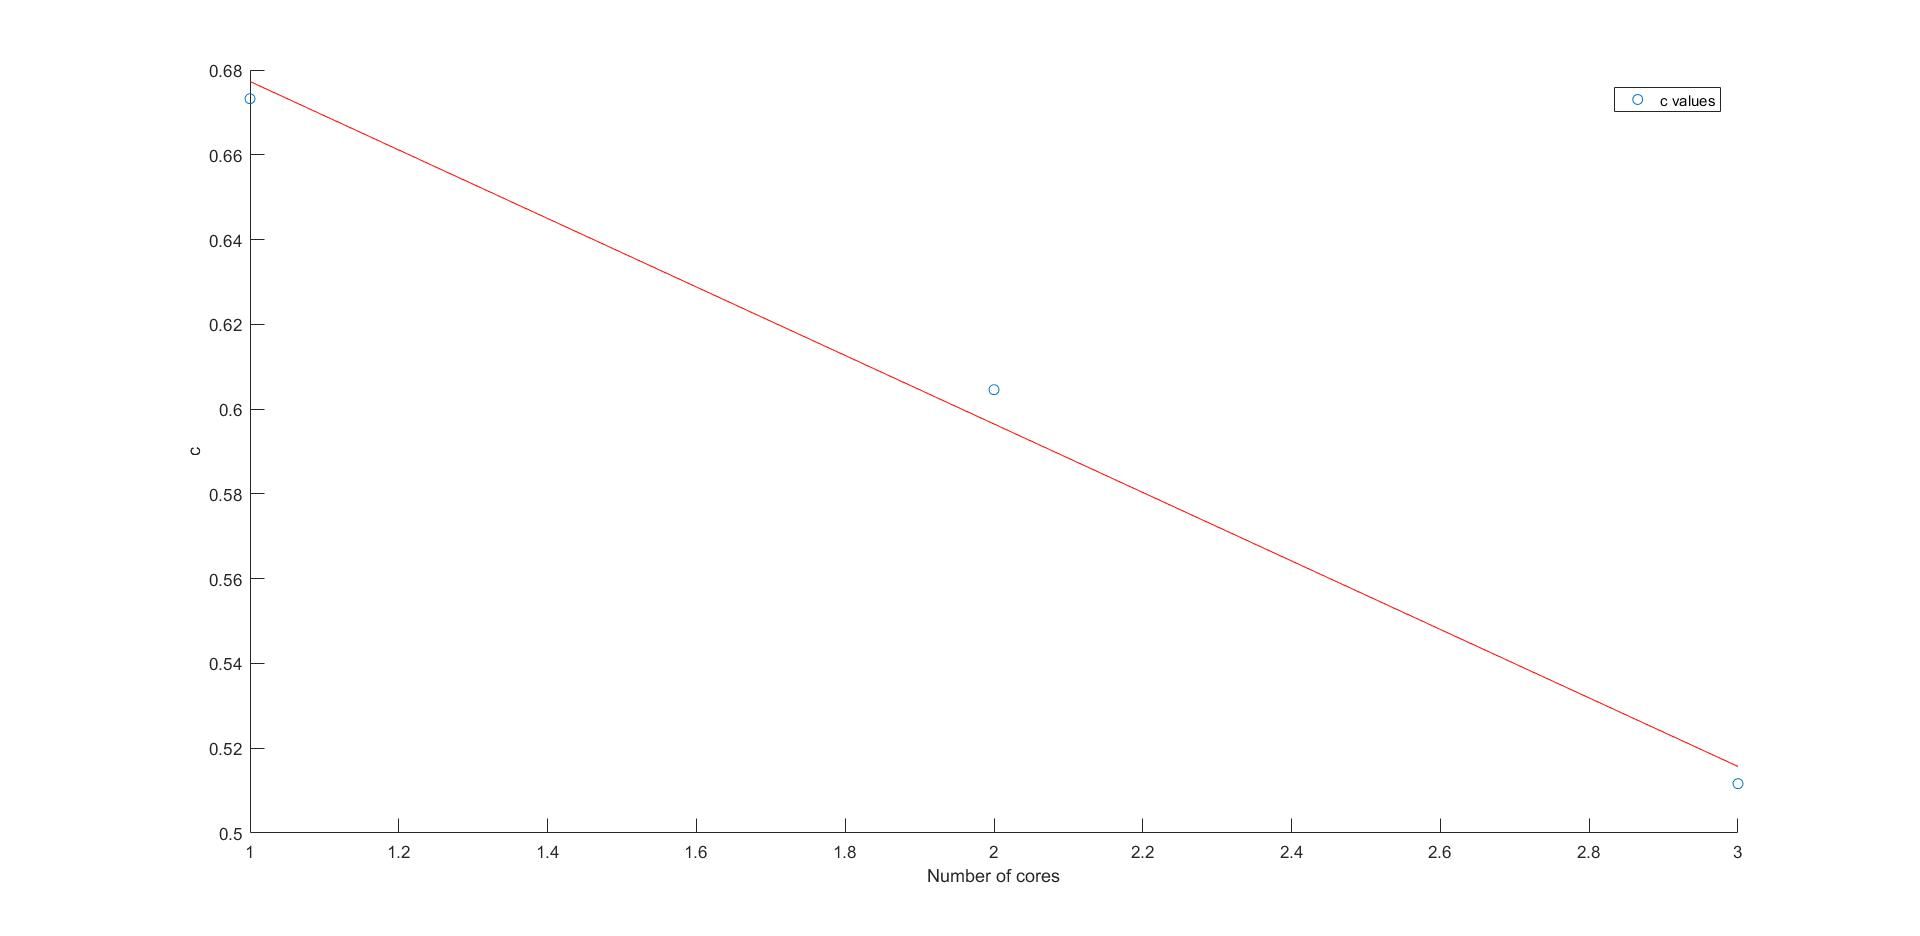
\includegraphics[scale=0.3]{images/dfe_c}
	\caption{$c$ against Number of cores}
\end{figure}

\noindent Similar to the multicore CPU, I chose to model $c$ using a linear function. 

\begin{equation}
y=-0.08079x+0.7581
\end{equation}

\noindent Comparing the equations for $a$, $b$ and $c$ for both the multicore CPU and multiDFEs, it seems that the equation for $b$ is of a different form. This means that the performance model for multicore compute nodes have to be represented by both the equations for $a$, $b$ and $c$ and their respective coefficients instead of just a set of coefficients for the $a$, $b$ and $c$ equations. Nevertheless, it should still be possible to model DFEs in a similar way that the multicore CPU is modelled, that is, model multiple DFEs as a single node with the power calculated using the equation corresponding to the number of DFEs, provided the simulation is intended to be used for expermentations that are out of the capabilities of the hardware resources available.

\subsection{CPU + DFE topology}
With the data obtained from the previous two subsection, I modelled the AdPredictor application for a simple CPU + DFE topology on the maxnode2 platform in SimGrid using the SimDAG API. The topology is displayed in Figure 10.

\begin{figure}[H]
	\centering
	\includegraphics[scale=0.5]{images/CPUDFEtopology}
	\caption{CPU + DFE topology}
\end{figure}

\noindent The simulation model can assign any number of tasks to the CPU node and DFE node and run the simulation. The twenty-four core CPU and four DFE nodes are represented by one compute node each in the platform configuration file and their throughputs are calculated programmatically using the equations obtained from subsections 3.1 and 3.2. This simulation allows the user to specify the amount of tasks to be computed by the CPU node as well as the number of cores to be used to compute the task and the same for the DFE node, to obtain the performance for the desired workload allocation.
\\\\
\noindent This can be very useful as it allows the user to select the best partition of a given workload size. For example, for the AdPredictor application, given a workload of 1000000 adimpressions, allocating 142000 adimpressions to twenty-four CPU cores and 878000 adimpressions to four DFEs would complete in the shortest amount of time. Using the simulation model, the user can test many different partition scenarios in a short amount of time.

\subsection{Modelling a DFE}

\section{Evaluation}
The error that comes with this method could potentially be quite large as there are many curve fittings. MATLAB provides the goodness of fit for each of these 'fit objects' which includes the sum of squares due to error (sse), R-squared (coefficient of determination), degrees of freedom in the error (dfe), degrees of freedom adjusted coefficient of determination (adjrsquare) and root mean squared error (rmse). 
\bibliographystyle{plain}

\begin{thebibliography}{9}

\bibitem{dataflow}
Maxeler Technologies, 2015. Multiscale Dataflow Programming Version 2015.1.1.
\bibitem{simulation}
Casanova, H., Giersch, A., Legrand, A., Quinson, M. and Suter, F., 2014. Versatile, scalable, and accurate simulation of distributed applications and platforms. Journal of Parallel and Distributed Computing, 74(10), pp.2899-2917.

\bibitem{simgrid}
Home. 2016. Home. [ONLINE] Available at: \url{http://simgrid.gforge.inria.fr/}. [Accessed 09 June 2016].
\end{thebibliography}

\end{document}

